\documentclass[11pt]{article}
\usepackage[utf8]{inputenc}
\usepackage[margin=1in]{geometry}
\usepackage{booktabs}
\usepackage{longtable}
\usepackage{graphicx}
\usepackage{hyperref}
\usepackage{float}
\hypersetup{
    colorlinks=true,
    linkcolor=blue,
    urlcolor=blue,
    citecolor=blue
}
\title{Indoor Greenhouse Robot Experiments}
\author{Raz Turgeman}
\date{\today}

\begin{document}
\maketitle

\section{Project Background and Integration}

This project is based on the \href{https://github.com/RoverRobotics/roverrobotics_ros2/tree/humble}{RoverRobotics Repo}, which provides all necessary infrastructure such as robot control, simulation in Gazebo, visualization in RViz, hardware interface, navigation, and SLAM. \\
The current work is connected to my own \href{https://github.com/RazTurgeman97/rover_volkani/tree/main}{Project's Repo}.

\subsection{Problems Addressed}
\begin{itemize}
    \item \textbf{Fixed SLAM Mapping Malfunction:} \\
    \textit{Issue:} The map rotated with the rover, making it unreadable. \\
    \textit{Cause:} The EKF relied only on missing camera/IMU data for yaw velocity. \\
    \textit{Fix:} Added yaw-velocity calculation from odometry. \\
    \item \textbf{Fixed Missing Rotation Recognition in Simulation:} \\
    Same root cause and fix as the SLAM issue — yaw velocity is now estimated from odometry.
    \item \textbf{Fixed Wheel Lock on Boot:} \\
    \textit{Issue:} Wheels locked immediately after boot due to a startup service suggested by the manufacturer. \\
    \textit{Fix:} Removed the conflicting service. \\
    \textit{Future:} Investigate the service’s purpose and re-integrate properly if needed.
\end{itemize}
Additionally, I added an IMU BNO055 component for improved odometry and localization results and utilized an Extended Kalman Filter (EKF) with the encoder sensor.

\subsection{Project Overview}

The goal of this project is to drive a robot in greenhouses to monitor plant diseases. Experiments are currently being conducted both indoors and outdoors using three rows of fake plants to simulate greenhouse conditions, with five plants per row.

\subsubsection{Environment and Equipment}
\textbf{System:} Ubuntu 22.04, ROS 2 Humble. \\
\textbf{Sensors:} Lidar S2 and IMU BNO055. \\
The indoor environment was scanned and named "indoor\_abc\_lab3". Each plant inception is considered as a 3-second stop next to the plant, either to the left or right of the robot.

\subsection{Experiment Goals}

\textbf{Indoor Experiments:}
\begin{itemize}
    \item \textbf{Experiment 1:} Stop next to each plant.
    \item \textbf{Experiment 2:} Stop next to each second plant.
    \item \textbf{Experiment 3:} Stop next to each $n$-th plant ($n$ is a user-supplied argument, different each time).
    \item \textbf{Experiment 4:} Stop next to five predetermined plants considered infected.
    \item \textbf{Experiment 5:} Stop next to each post-determined (after the robot starts "checking" plants, live push data of an infected plant in real-time) infected plant from $m$ infected plants, and for each $i$ from $m$ infected plants, check the $j+1$ and $j-1$ plants (the plants before and after the infected plant row) for disease spread.
\end{itemize}

There should be three levels of infection: 10\%, 25\%, and 50\%.

Each experiment is to be conducted three times, both with and without the IMU.

Thus, $5$ experiments $\times$ $3$ repeats $\times$ $2$ (with/without IMU) equals $30$ total experiments. \\

\textbf{Outdoor Experiments:}

The indoor process is to be repeated outdoors, resulting in another $30$ experiments.

\textbf{Total:} Indoor + Outdoor = $60$ experiments in total.

\subsection{Current Status}

At present, only indoor experiments with the IMU have been completed, without infection levels, in a simulation based on the real lab lidar scan. A Gazebo world was created based on the lidar map as well. \\
Experiments 1–4 were conducted, with three attempts for each experiment, totaling $12$ experiments.
Due to the war situation, the experiments were carried out only in simulation.

\section{Overview}
I ran four different “snake” pattern navigation experiments in a Gazebo indoor greenhouse.  In each run the robot visits plant centers in the order 
1→5→10→6→11→15, but stops at different subsets depending on the experiment type:

\begin{center}
\begin{tabular}{@{}cl@{}}
\toprule
\textbf{Experiment Type} & \textbf{Description} \\
\midrule
1 & Stop at \emph{every} plant (IDs 1,2,3,4,5,10,9,8,7,6,11,12,13,14,15) \\
2 & Stop at \emph{every 2nd} plant\\
3 & Stop at \emph{every 3rd} plant \\
4 & Stop at \emph{predetermined} plants (user-supplied) \\
\bottomrule
\end{tabular}
\end{center}

Each experiment was repeated {\bf three} times to gauge repeatability.

\section{Commands \& Launch Files}
\subsection{Gazebo Simulation}
\begin{verbatim}
ros2 launch roverrobotics_gazebo 2wd_rover_indoor_lab.launch.py
\end{verbatim}

\subsection{Navigation Stack}
\begin{verbatim}
ros2 launch roverrobotics_driver navigation_launch.py
\end{verbatim}

\subsection{Run a Specific Experiment}
\begin{verbatim}
ros2 run roverrobotics_driver greenhouse_experiment_node --ros-args
-p experiment_type:=<1|2|3|4>
\end{verbatim}

\subsection{Post-process Results}
\begin{verbatim}
ros2 run experiment_monitor experiment_monitor --ros-args
-p experiment_type:=<1|2|3|4>
\end{verbatim}

Replace \texttt{<1|2|3|4>} with the desired experiment type.

\section{Key Results}
Below are the aggregate statistics (mean ± std over three attempts) for each experiment type:


\begin{table}[H]
\centering
\begin{tabular}{@{}lccccc@{}}
\toprule
\textbf{Exp} & \textbf{Mean task dur [s]} & \textbf{Std dur [s]} 
            & \textbf{Mean error [m]}  & \textbf{Std err [m]} & \textbf{Success \%} \\
\midrule
1 (all)           & 13.3  & 3.7  & 0.19  & 0.004 & 100\,\% \\
2 (every second)  & 23.4  & 7.0  & 0.19  & 0.041 &  98\,\% \\
3 (every third)   & 24.7  & 13.1 & 0.18  & 0.011 & 100\,\% \\
4 (predetermined) & 32.1  & 7.9  & 0.18  & 0.014 & 100\,\% \\
\bottomrule
\end{tabular}
\caption{Mean ± std across three attempts per experiment.}
\end{table}

\bigskip
\noindent

\section{Experiment Visualizations}

\begin{figure}[H]
    \centering
    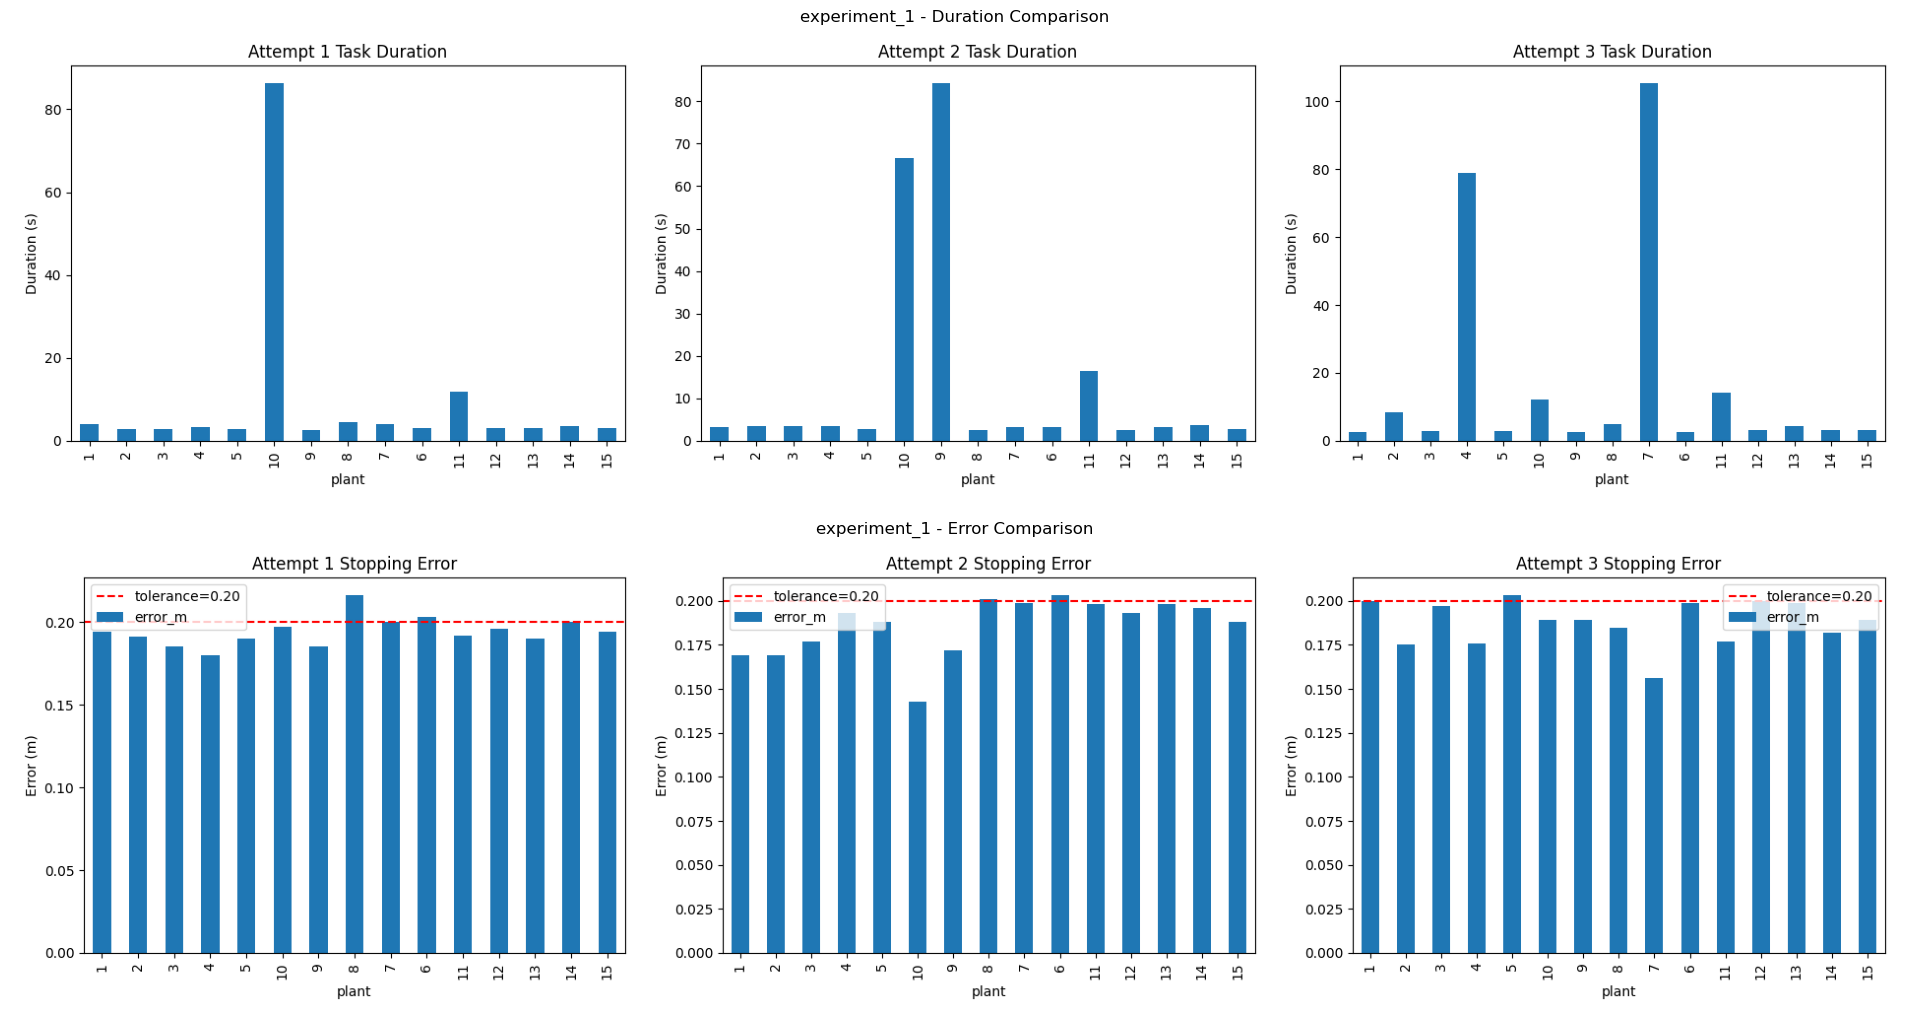
\includegraphics[width=1.0\textwidth]{images/comparison_all_1.png}
    \caption{Experiment Type 1: Stop at every plant.}
    \label{fig:exp1}
\end{figure}

\begin{figure}[H]
    \centering
    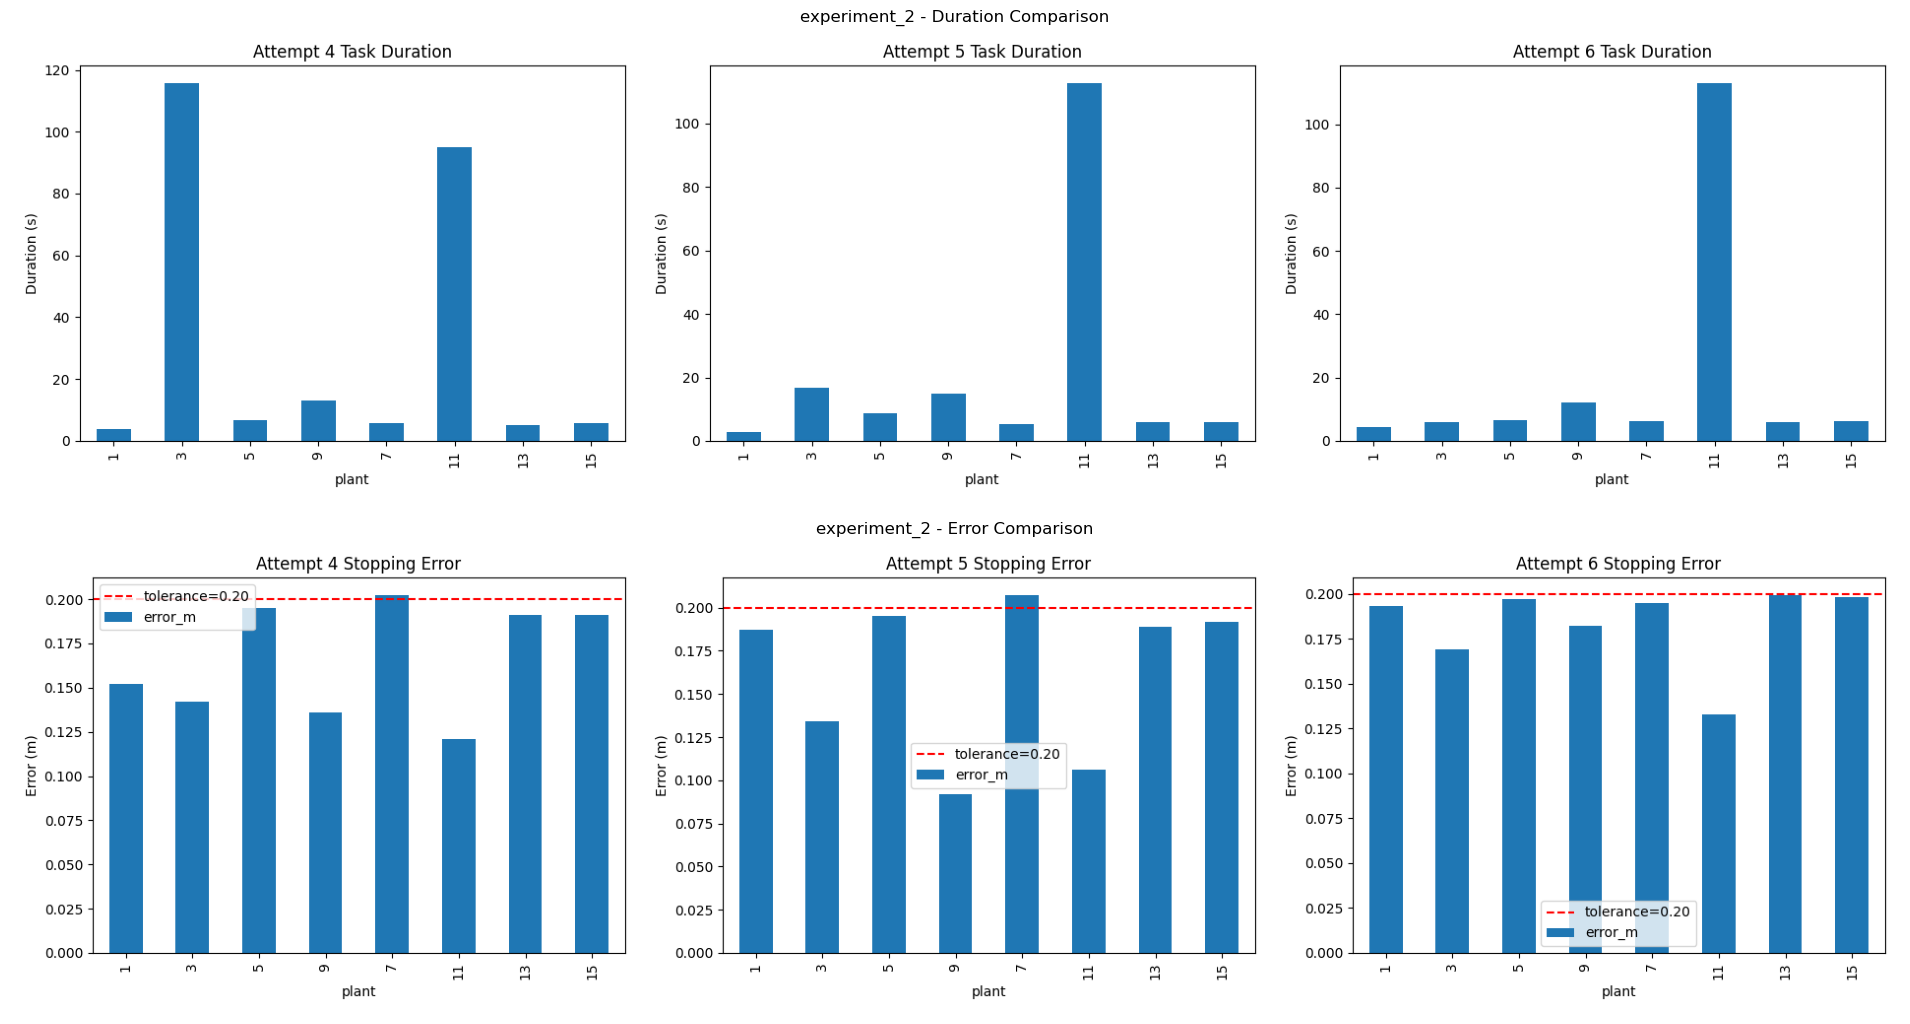
\includegraphics[width=1.0\textwidth]{images/comparison_all_2.png}
    \caption{Experiment Type 2: Stop at every 2nd plant.}
    \label{fig:exp2}
\end{figure}

\begin{figure}[H]
    \centering
    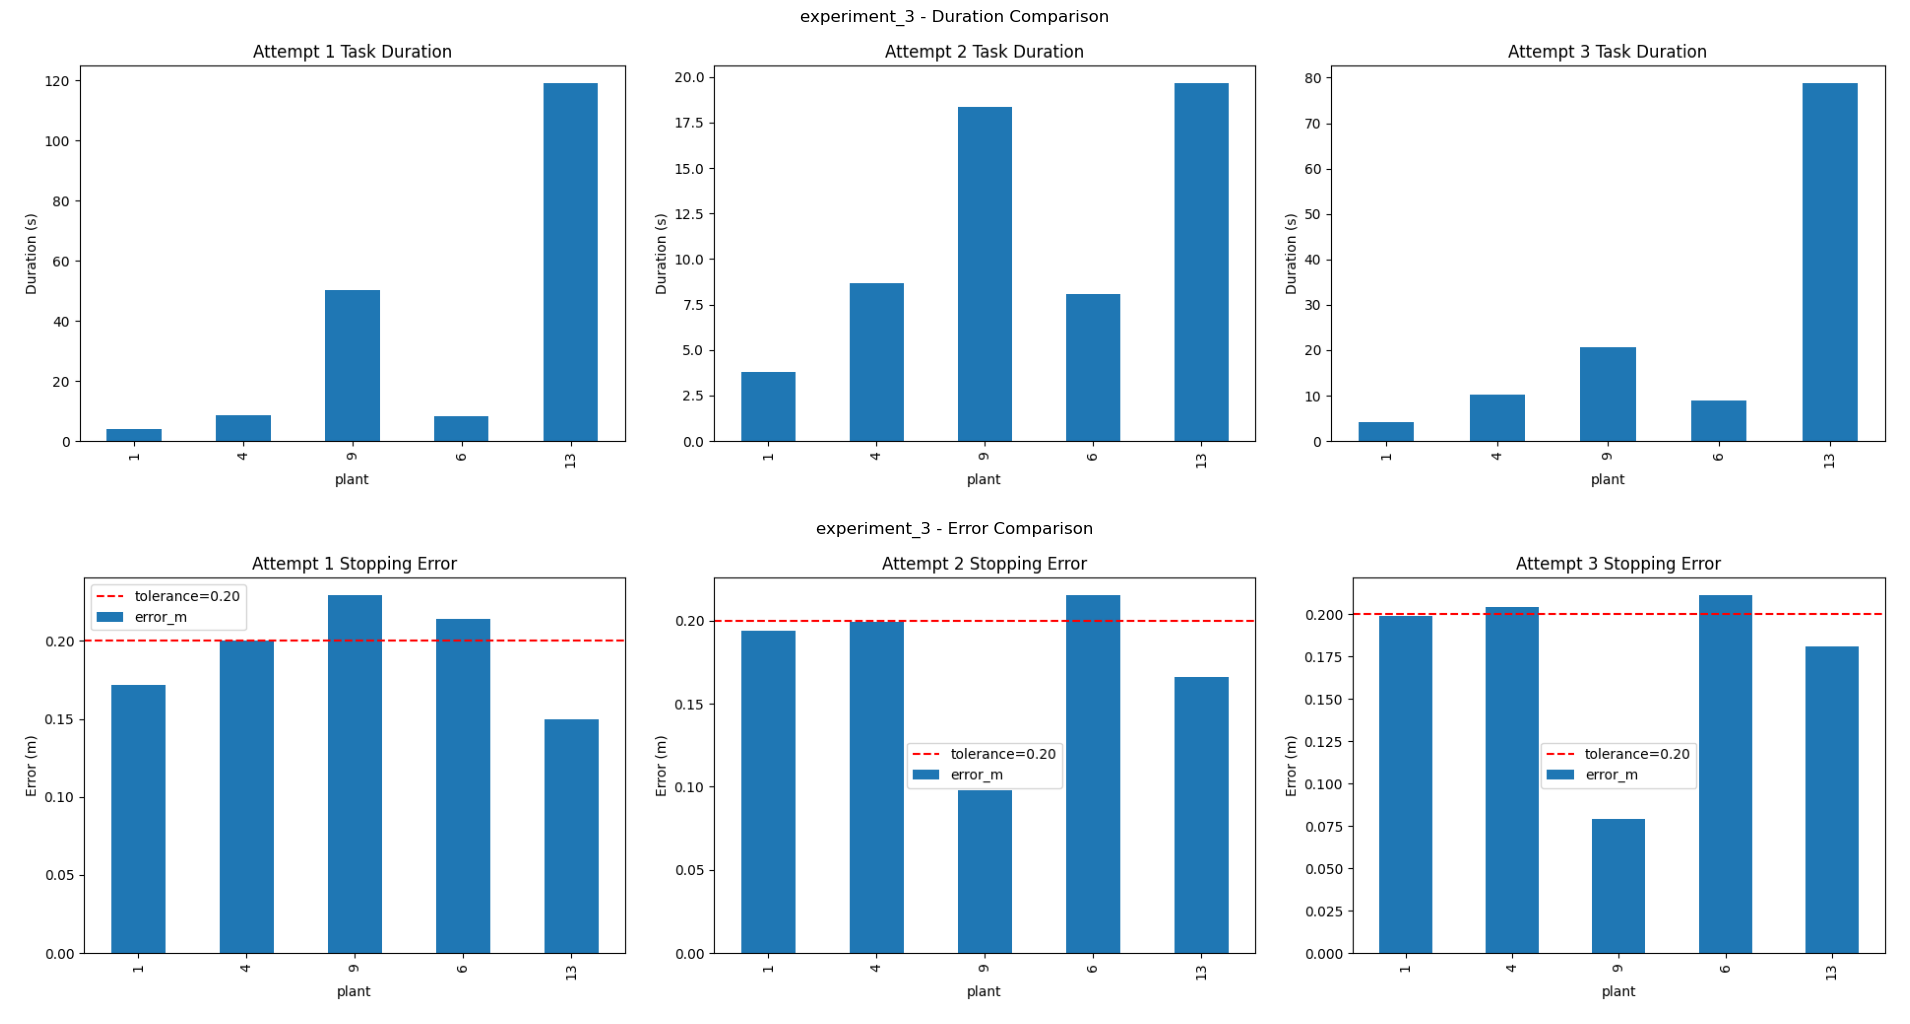
\includegraphics[width=1.0\textwidth]{images/comparison_all_3.png}
    \caption{Experiment Type 3: Stop at every 3rd plant.}
    \label{fig:exp3}
\end{figure}

\begin{figure}[H]
    \centering
    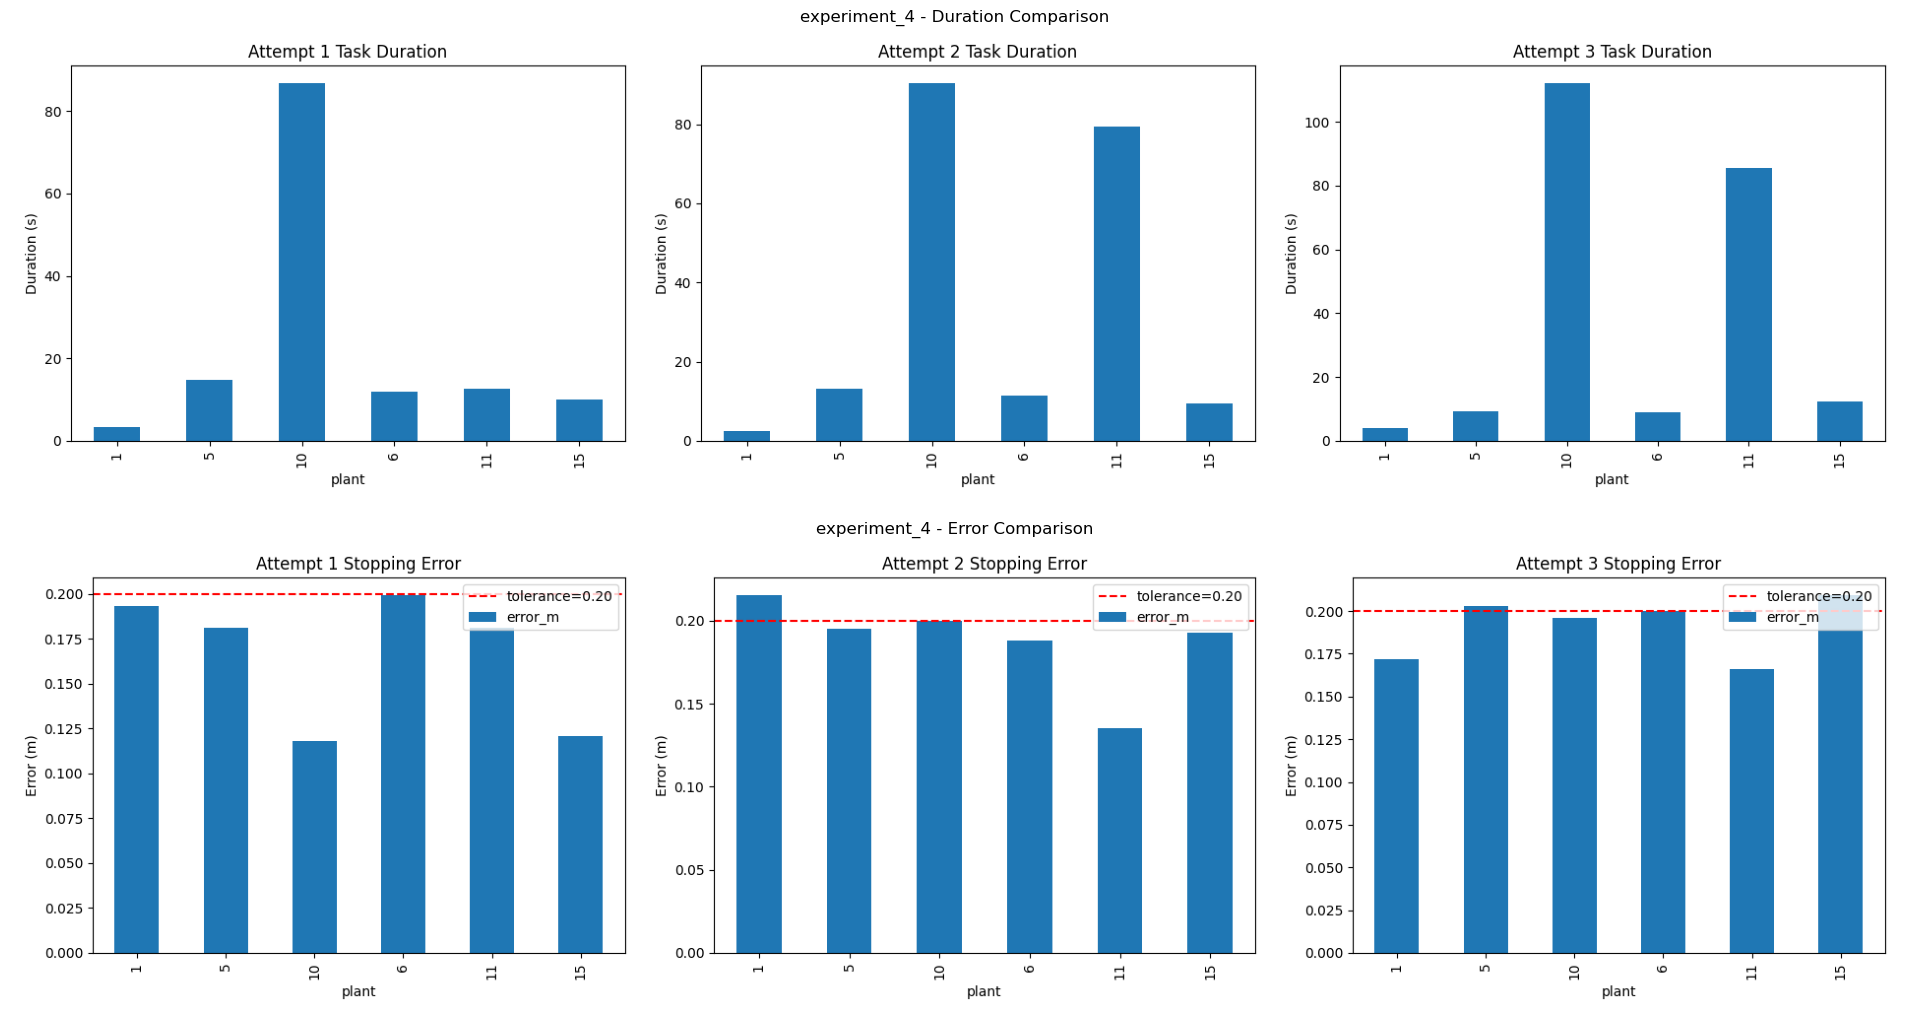
\includegraphics[width=1.0\textwidth]{images/comparison_all_4.png}
    \caption{Experiment Type 4: Stop at predetermined plants.}
    \label{fig:exp4}
\end{figure}

\section{Experiment Situations and Notable Events}

This section presents selected situations and notable events encountered during the experiments. Each image illustrates a specific scenario, as described in its caption.

\begin{figure}[H]
    \centering
    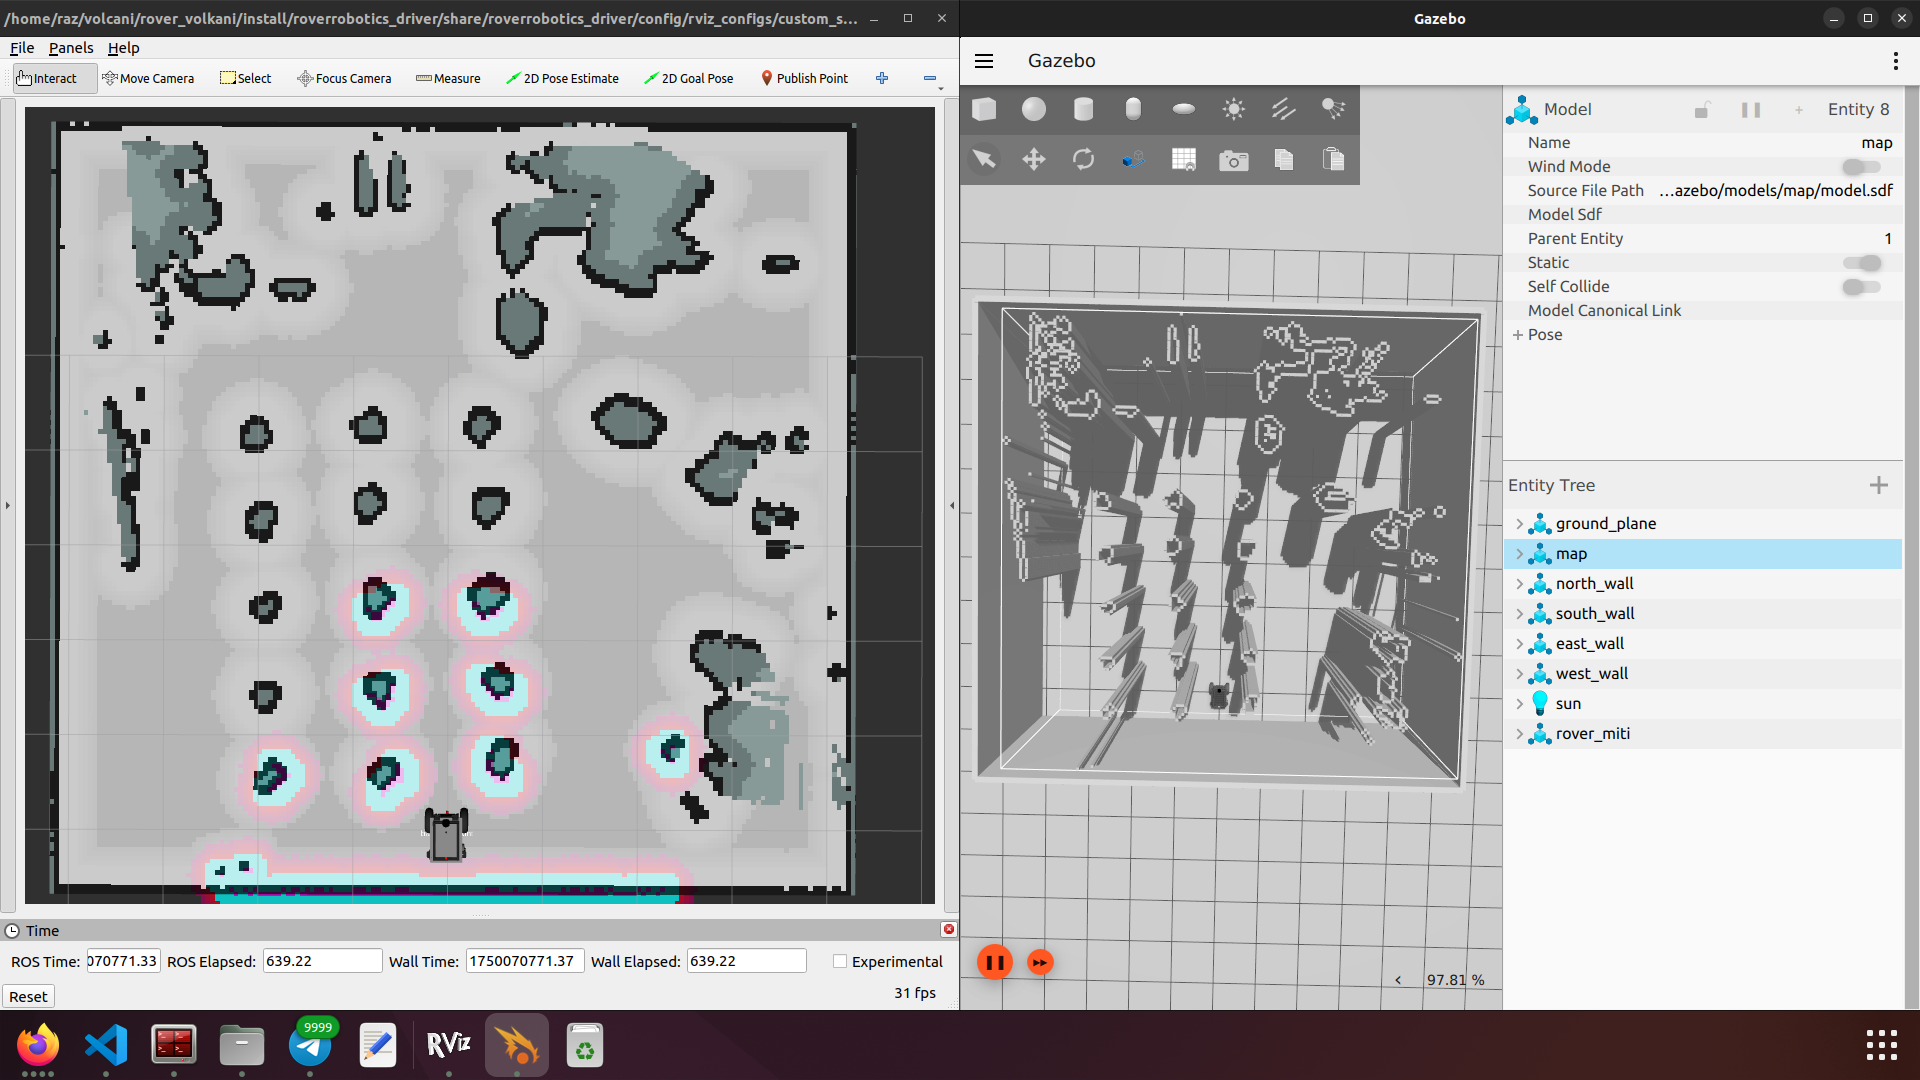
\includegraphics[width=0.8\textwidth]{images/experiment home.png}
    \caption{Home position: The robot's initial position in the experiment environment.}
\end{figure}

\begin{figure}[H]
    \centering
    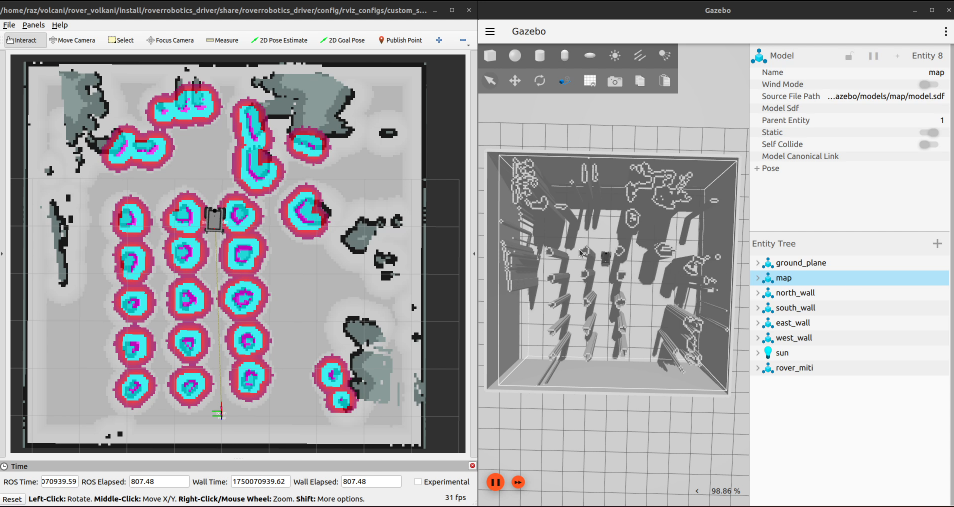
\includegraphics[width=0.8\textwidth]{images/experiment cost map.png}
    \caption{Cost map visualization: The cost map used by the navigation stack, showing obstacles and planned paths.}
\end{figure}

\begin{figure}[H]
    \centering
    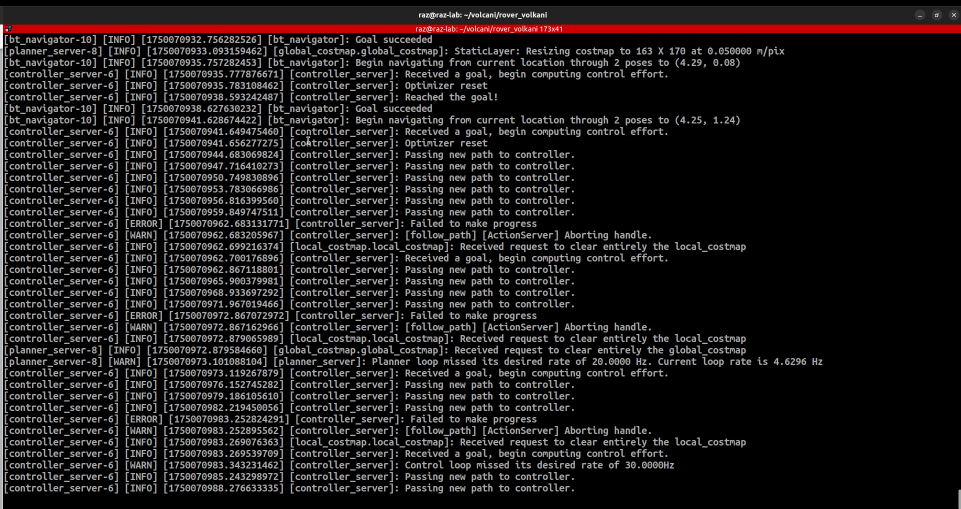
\includegraphics[width=0.8\textwidth]{images/experiment 1 plant 10 long stay - log.png}
    \caption{Experiment 1: The robot performed a prolonged stop at plant 10, as seen in the log. This may indicate a navigation or detection delay at this plant.}
\end{figure}

\begin{figure}[H]
    \centering
    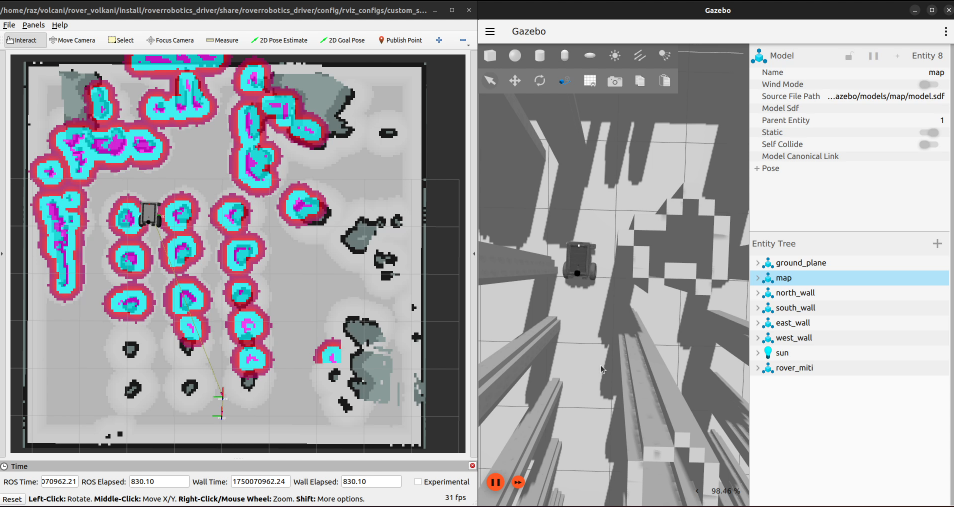
\includegraphics[width=0.8\textwidth]{images/experiment 1 plant 10 long stay - sim.png}
    \caption{Experiment 1: Simulation view of the robot's long stay at plant 10, confirming the behavior observed in the log.}
\end{figure}

\begin{figure}[H]
    \centering
    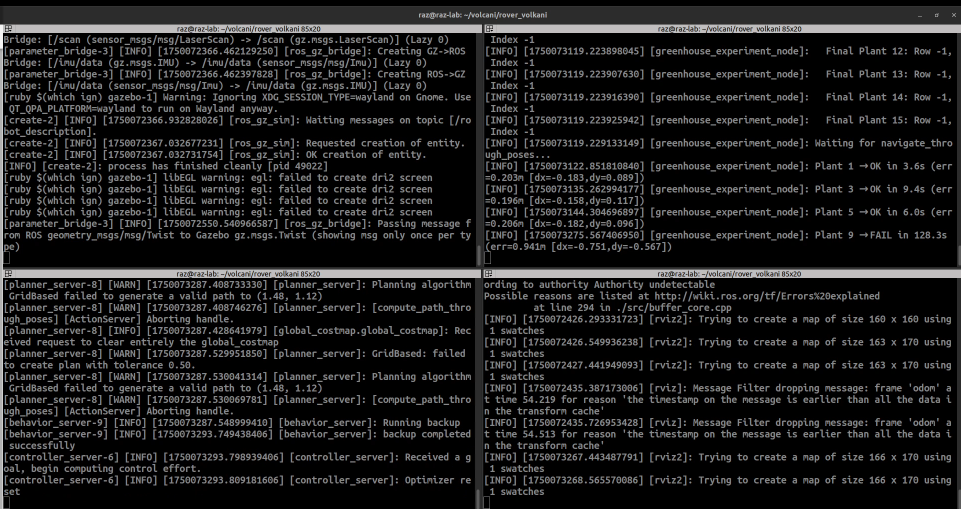
\includegraphics[width=0.8\textwidth]{images/experiment 2 - plant 9 fail due to collision - log.png}
    \caption{Experiment 2: Failure at plant 9 due to a collision, as recorded in the log. The robot was unable to complete its approach.}
\end{figure}

\begin{figure}[H]
    \centering
    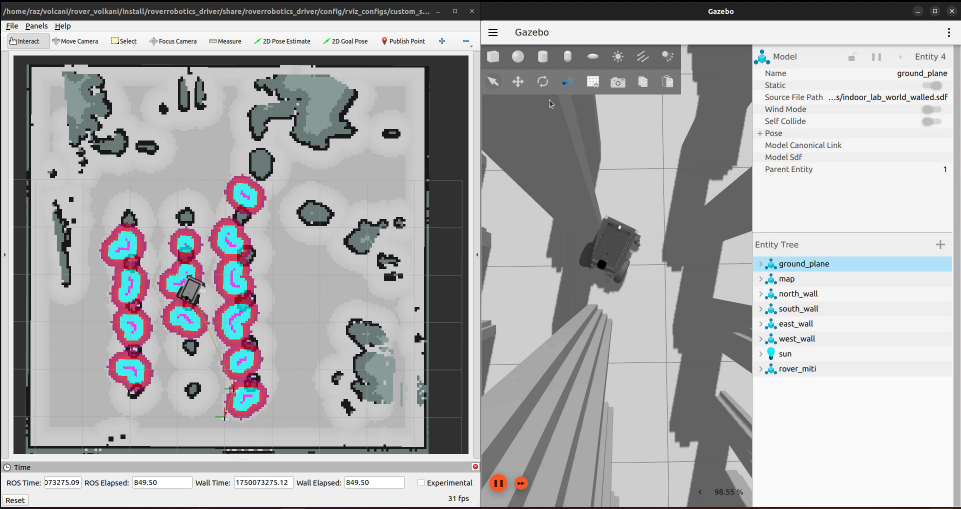
\includegraphics[width=0.8\textwidth]{images/experiment 2 - plant 9 fail due to collision -sim.png}
    \caption{Experiment 2: Simulation snapshot of the collision event at plant 9, showing the robot's position at the time of failure.}
\end{figure}

\begin{figure}[H]
    \centering
    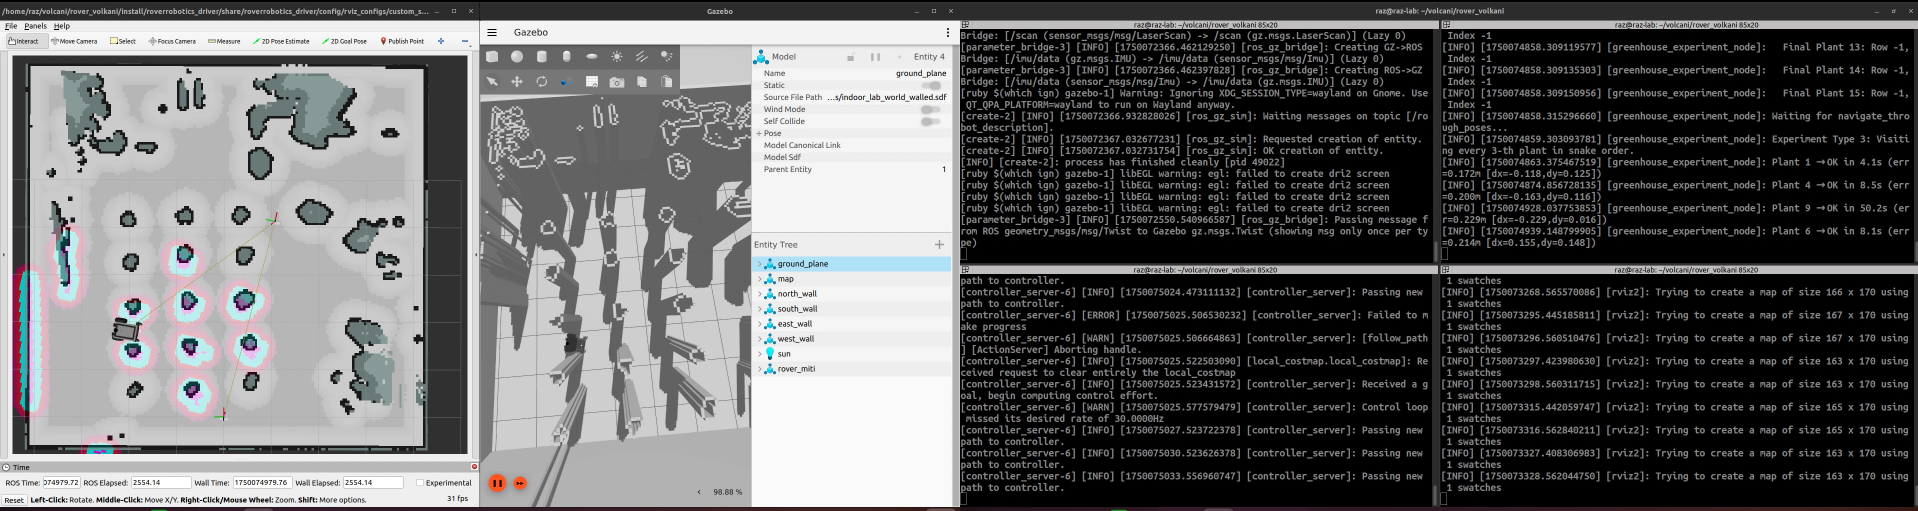
\includegraphics[width=1\textwidth]{images/experiment 3 - unwanted path in the middle of raw 3 - sim + log.png}
    \caption{Experiment 3: The robot followed an unwanted path in the middle of row 3, as shown by both simulation and log data. This highlights a navigation anomaly.}
\end{figure}

\begin{figure}[H]
    \centering
    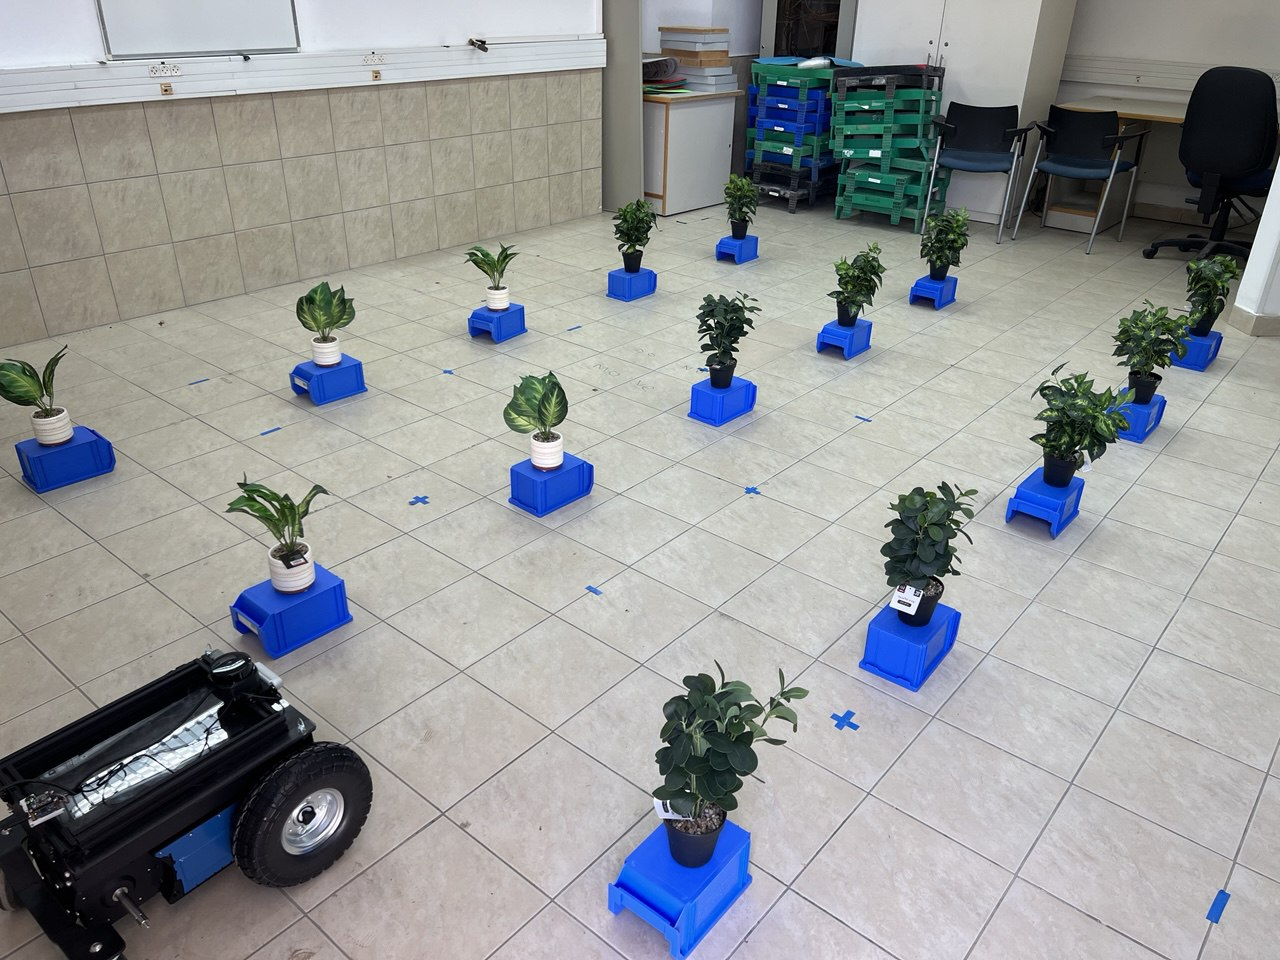
\includegraphics[width=0.8\textwidth]{images/Indoor Experiment Environment.jpg}
    \caption{Indoor experiment environment: Overview of the Real greenhouse setup used for the experiments.}
\end{figure}

\end{document}
